\documentclass[12pt, titlepage]{article}

\usepackage{booktabs}
\usepackage{tabularx}
\usepackage{hyperref}
\usepackage{float}
\usepackage{graphicx}
\hypersetup{
    colorlinks,
    citecolor=black,
    filecolor=black,
    linkcolor=red,
    urlcolor=blue
}
\usepackage[round]{natbib}
\usepackage{array}

\title{SE 3XA3: Software Requirements Specification\\Title of Project}

\author{Team \#104
		\\ Andrew Hum, 400138826
		\\ Arshan Khan, 400145605
		\\ Jame Tran, 400144141
		\\ William Lei, 400125240
}

\date{\today}

%\input{../Comments}

\begin{document}

\maketitle

\pagenumbering{roman}
\tableofcontents
\listoftables

\begin{itemize}
\item Table 1: Revision History
\item Table 2: Work Partitioning Events
\item Table 3: Work Partitioning Event Summaries
\end{itemize}

\listoffigures

\begin{itemize}
    \item Figure 1: System Use Case Diagram
\end{itemize}

\begin{table}[bp]
\caption{\bf Revision History}
\begin{tabularx}{\textwidth}{p{3cm}p{2cm}X}
\toprule {\bf Date} & {\bf Version} & {\bf Notes}\\
\midrule
2/3/2020 & 1.0 & Project Drivers and Project Issues\\
2/8/2020 & 1.1 & Completed Functional Requirements\\
2/8/2020 & 1.2 & Completed Non Functional Requirements\\
2/9/2020 & 1.3 & Final Revision\\

\bottomrule
\end{tabularx}
\end{table}

\newpage

\pagenumbering{arabic}

%This document describes the requirements for ....  The template for the Software Requirements Specification (SRS) is a subset of the Volere template~\citep{RobertsonAndRobertson2012}.  If you make further modifications to the template, you should explicitly state what modifications were made.

\section{Project Drivers}

\subsection{The Purpose of the Project}

For all time, humans have played games for entertainment, as a pass-time, and as a way to relieve stress. In the last few decades, humans have had the ability to create games that run on the computer as well. Over time, these games have only improved in their complexity and design, as well as generated billions of dollars in revenue for the entire gaming industry. Our focus is not on profit however, we care most about giving the players a seamless, satisfying experience when playing the mini games. Thus, we are focusing on making visual and difficulty enhancements to a pre-existing set of mini games.

\subsection{The Stakeholders}

\subsubsection{The Client}

\begin{itemize}
    \item The clients for the product are Dr. Asghar Bokhari and the SFWRENG 3XA3 Teaching Assistants. As clients, they will administer the development of the product as well as offer assistance and clarification wherever possible. They will also determine the degree to what the product delivers on the requirements.
\end{itemize}

\subsubsection{The Customers}

The intended customers of the product are any individuals with the ability to download the product online. This includes a child, up to a senior citizen. The product is created to entertain its users and give them a joyful experience.

\subsubsection{Other Stakeholders}

All other stakeholders include all current developers as well as any future developers who wish to further improve upon the open-source project themselves.

\subsection{Mandated Constraints}

The system is to be built under the following constraints

\begin{itemize}
    \item The product must run successfully on at least Windows and MacOS.
    \item The product must be able to be installed in less than 30 minutes by only installing the executable file.
    \item The product must not require any specialized hardware which the common user may not have.
    \item The product must free of cost to all users.
    \item The product must be sufficiently complete by March 20, 2020.
    \item The product must contain at least one playable mini-game.
    \item Development cost of the product must not exceed \$0.
    \item The mini-game(s) must have a visual and/or difficulty improvement to be considered "updated".
\end{itemize}

\subsection{Naming Conventions and Terminology}

Not applicable.

\subsection{Relevant Facts and Assumptions}

It is assumed that the pygame and/or the tkinter libraries are sufficient to update the mini games. Also, the mini games will be either visually enhanced or with new difficulty levels; both will be true only if time permits the developers to achieve this.

\section{Functional Requirements}

\subsection{The Scope of the Work and the Product}

The Current Situation:

\begin{itemize}
    \item Currently no launcher. To run the games you need to install the code from using Ubuntu, and running each game individually.
    \item Maze: a minimal 2-dimensional maze with one preset maze that is generated that can be navigated through single mouse clicks with little-to-no difficulty.
    \item Flappy: a simplistic game where the user utilizes the mouse-click to prevent their character from colliding with randomly generated objects, and loses when the collide
    \item Pong: a very simple version of the classic game Pong. It is a two-player game that has contains minimal physics aspect as well as poor graphics and poor performance.
\end{itemize}

\subsubsection{The Context of the Work}
\begin{itemize}
    \item This mini game launcher is developed for the course, SFWRENG 3XA3, professor Dr. Asghar Bokahri and the teaching assistants assigned to our group, Thien Tandinh and Oluwaseum Owojaiye.
\end{itemize}
\subsubsection{Work Partitioning}

\begin{table}[H]
\caption{Work Partitioning Events}
\begin{center}
\setlength{\tabcolsep}{3pt}
\resizebox{\linewidth}{!}{%
\begin{tabular}{|c|c|c|c|}
\hline
Event Number & Event Name & Input & Output \\
\hline
1 & Selecting/Launching a Game & Mouse/Keyboard & Selected Game \\
\hline
2 & Accessing the Leader-boards & Mouse/Keyboard & Display Leader-board\\
\hline
3 & Playing the Maze & Keyboard & Final Score\\
\hline
4 & Playing Flappy & Keyboard & Final Score\\
\hline
5 & Playing Pong & Keyboard & Final Score\\
\hline
\end{tabular}%
}
\end{center}
\label{wpe}
\end{table}%

\begin{table}[H]
\caption{Work Partitioning Event Summaries}
\begin{center}
\setlength{\tabcolsep}{3pt}
\resizebox{\linewidth}{!}{%
\begin{tabular}{|c|c|}
\hline
Event Number & Summary\\
\hline
1 & Based on the user’s input, launch the specified game\\
\hline
2 & If the user chooses to access the leader-board, a list of the high\\ &scores will be listed and will have the option to be sorted by each\\ &game.\\
\hline
3 & The user will select the difficulty of the maze and navigate their\\ &object through the maze using the keyboard. Once completed the system\\ &will provide the user with their final score which is the time it took\\ &to complete the maze.\\
\hline
4 & The user will start a new game and use the space-bar to avoid\\ &obstacles. The system will provide their final score once they collide\\ &with an obstacle based on the time elapsed.\\
\hline
5 & The user will use the keyboard to play against an opponent controlled\\ &by the system to try to score against them. They will play till\\ &either they or their opponent reaches a desired score. \\&The system will then display the final score and record their score.\\
\hline
\end{tabular}%
}
\end{center}
\label{wps}
\end{table}%


\subsubsection{Individual Product Use Cases}

\begin{figure}[H]
    \centering
    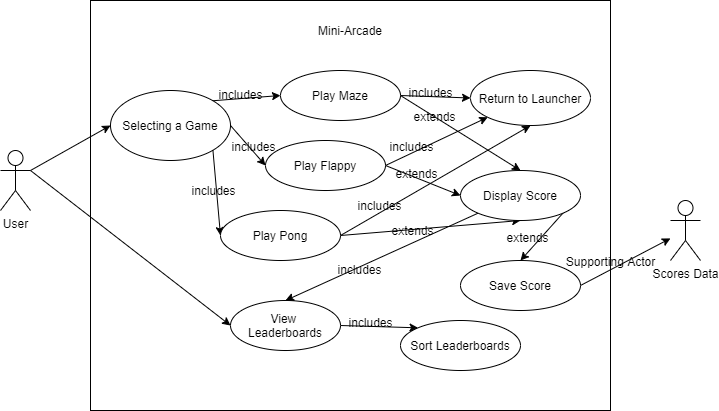
\includegraphics[width=6in]{Images/UseCaseDiagram.png} 
    \caption{System Use Case Diagram}
    \label{fig:example}
 \end{figure}
 

\subsection{Functional Requirements}
    BE1. The user wants to play a game
    \begin{itemize}
    \item FR1. The system shall provide the user with several different mini-game options
    \item FR2. The system shall launch the desired mini-game in the same window
    \item FR3. The system shall provide an option to close the application
    \end{itemize}
    BE2. The user wants to view their scores
    \begin{itemize}
        \item FR4. The system shall provide the user with the ability to view the leader-boards from the launcher
        \item FR5. The system shall provide the user with the ability to sort their scores based on the game
        \item FR6. The system shall provide the user the ability to view the current game’s leader-boards from the game home screen
    \end{itemize}
    BE3. The user wants to play Maze
    \begin{itemize}
        \item FR7. The system shall provide the user with different difficulty levels
        \item FR8. The system shall record the user’s current score based on the time elapsed
        \item FR9. The system shall randomly generate mazes based on difficulty
        \item FR10. The system shall provide a home button to exit the game at any time
        \item FR11. The system shall display the user’s current score and high score once the complete the maze
        \item FR12. The user shall be able to control the object’s movement with the keyboard
        \item FR13. The system shall provide an option to proceed to another maze once completed
        \item FR14. The system shall provide an option to return to the launcher
    \end{itemize}
    BE4. The user wants to play Flappy
    \begin{itemize}
        \item FR15. The system shall provide the user with the option to start a new game
        \item FR16. The user shall use the space-bar to control their character
        \item FR17. The system shall randomly generate objects to interfere with the character
        \item FR18. The system shall increase speed as the time elapsed increases
        \item FR19. The system shall generate more objects as the time elapsed increases
        \item FR20. The system shall provide the user with the final time elapsed once the game is over
        \item FR21. The system shall provide the option to view the score boards for Flappy
        \item FR22. The system shall provide the user the option to play again
        \item FR23. The system shall provide the user with the option to return to the launcher
    \end{itemize}
    BE5. The user wants to play Pong
    \begin{itemize}
        \item FR24. The system shall provide the user with the option to play alone or with a friend
        \item FR25. The user(s) shall use the keyboard to navigate their paddle(s)
        \item FR26. The system shall add a point to the side that scores
        \item FR27. The system shall require a final score to play up to
        \item FR28. The system shall end the game once the final score is reached by either side
        \item FR29. The system shall provide the option to play again
        \item FR30. The system shall provide the option to return to the launcher
    \end{itemize}


\section{Non-functional Requirements}
\subsection{Look and Feel Requirements}
NFR1
\begin{itemize}
    \item DESCRIPTION: The games should run at a suitable, fast, stable frame rate 
    \item RATIONALE: In order for the game's performance feels responsive and the animations feel "smooth", a high frame rate is needed
    \item FIT CRITERION: The game should run at a consistent 30 fps or more
    \item PRIORITY: HIGH
\end{itemize}

NFR2 
\begin{itemize}
    \item DESCRIPTION: The overall theme of our arcade app should be visually appealing
    \item RATIONALE: The colours of the games should capture the user's attention to keep their interest 
    \item FIT CRITERION: The colours used by our games should abide by the color theory, to ensure important areas of the game stands out.
    \item PRIORITY: HIGH
\end{itemize}


\subsection{Usability and Humanity Requirements}
NFR3
\begin{itemize}
    \item DESCRIPTION: The UI should be non intrusive and easy to use
    \item RATIONALE: In a fast paced, competitive game the UI should interfere with the user's 
ability to play the game as little as possible.
    \item FIT CRITERION: Ensure that most of the screen is dedicated to the game-play elements
of the game
    \item PRIORITY: HIGH
\end{itemize}

NFR4
\begin{itemize}
    \item DESCRIPTION: The game-play should be intuitive and easy to learn with minimal instructions
    \item RATIONALE: In order to attract an international user-base, the games should be very
easy understand with minimal English instructions
    \item FIT CRITERION: The game should use pictorial tutorials, have easy to understand game-play
and appropriate visual effects
    \item PRIORITY: MEDIUM
\end{itemize}

\subsection{Performance Requirements}
NFR5
\begin{itemize}
    \item DESCRIPTION: The game should load quickly and effortlessly
    \item RATIONALE: In order to ensure a good user experience, the app should keep any
"non gaming" time to a minimum.
    \item FIT CRITERION: Ensure that the game is properly optimized to keep loading times under
20 seconds.
    \item PRIORITY: MEDIUM
\end{itemize}

NFR6
\begin{itemize}
    \item DESCRIPTION: The game should have minimal input lag.
    \item RATIONALE: To avoid latency/discrepancies between what the user sees and what the user is doing,
input lag should be minimized as much as possible.
    \item FIT CRITERION: Ensure that the game is updated within a quarter of a second of user input.
    \item PRIORITY: HIGH
\end{itemize}

\subsection{Operational and Environmental Requirements}
NFR7
\begin{itemize}
    \item DESCRIPTION: The arcade app should be easily accessible to the end user on any OS and machine
    \item RATIONALE: Many end users will have a wide variety of computers with different processors and OSs
    \item FIT CRITERION: The arcade app needs to be able to run on a wide variety of end user
computers
    \item PRIORITY: HIGH
\end{itemize}

\subsection{Maintainability and Support Requirements}
NFR8
\begin{itemize}
    \item DESCRIPTION:  Maintenance should be kept to a minimum.
    \item RATIONALE: Maintenance of the app will be kept to a minimum, in order to not
intefere with the user or to split the user-base between different software versions.
    \item FIT CRITERION: The game arcade app should be released with at least 90% of errors resolved.
    \item PRIORITY: LOW
\end{itemize}

\subsection{Security Requirements}
NFR9
\begin{itemize}
    \item DESCRIPTION: Games app should not allow players to modify any in game data, attributes or properties 
that are not intended to be tampered with.
    \item RATIONALE:  Cheating should be prohibited in a competitive setting.
    \item FIT CRITERION: An experienced player should know the result of any actions in the game.
    \item PRIORITY: LOW
\end{itemize}

\subsection{Cultural Requirements}
NFR10
\begin{itemize}
    \item DESCRIPTION: The product will not purposefully be offensive to any religious or ethnic group.
    \item RATIONALE: Being offensive to any racial or religious groups will limit the player base.
    \item FIT CRITERION: The content of the game will not include any material that may be offensive to any religious or ethnic groups.
    \item PRIORITY: HIGH
\end{itemize}
\subsection{Legal Requirements}
NFR11
\begin{itemize}
    \item DESCRIPTION: The product must not break the law.
    \item RATIONALE: Mini-Arcade must not break the law.
    \item FIT CRITERION: Do not break any laws.
    \item PRIORITY: HIGH
\end{itemize}

\subsection{Health and Safety Requirements}
NFR12
\begin{itemize}
    \item DESCRIPTION: The product must not cause any adverse health effects.
    \item RATIONALE: Playing games on a screen can cause various injuries, such as repetitive strain injuries
or eye strain which we should take care to avoid.
    \item FIT CRITERION: We will have popups to alert the user that they should take a 
break after an extended period of play (1 hour or more)
    \item PRIORITY: MEDIUM
\end{itemize}

This section is not in the original Volere template, but health and safety are
issues that should be considered for every engineering project.

\section{Project Issues}

\subsection{Open Issues}

The following describes issues that has been raised , but have not yet solved:
\begin{enumerate}
    \item The mini-games are currently using turtle as the graphic library, but the functionality turtle provides is very basic as it is designed as a introduction library for python beginners. Therefore a different graphic library is needed and the codes must be adjusted to use the new graphic library, preferably before any further development is done (this reduces the complexity of switching libraries).
\end{enumerate}

\subsection{Off-the-Shelf Solutions}

As some of the mini-games are based on commonly spread ideas, there is a decent amount of similar games out there, such as pac-man, flappy bird, pong, etc.

\subsection{New Problems}

Our project provide a all-in-one package to some of the common mini-games, with a standalone executable launcher providing access to multiple common mini-games without the need of external libraries and internet connection on computers.

\subsection{Tasks}

\begin{center}
\begin{tabular}{ |c|c| } 
\hline
\textbf{Task} & \textbf{Timeline}\\
\hline
Launcher Model Implementation and  & February 13\textsuperscript{th}\\
Partial Graphic Library Adaptation &\\
\hline
Adopt New Graphic Library & February 23\textsuperscript{th}\\
\hline
Launcher Development and Game Remake & March 15\textsuperscript{th}\\
\hline
Testing and Revision & March 29\textsuperscript{th}\\
\hline
\end{tabular}
\end{center}

\textcolor{white}{...}\\ %remove awkward indent
Task 1: Basic model for launcher and partially modify the mini-game to adapt with new graphic library (at least modify the main menu).\\
Task 2: Finish the adaptation to the new graphic library.\\
Task 3: Finish development of the launcher and remake the mini-games to provide more functionality to each mini-game.\\
Task 4: Test the launcher and mini-game, fix bugs found during testing and optimizes the mini-games.

\subsection{Migration to the New Product}

Not applicable.

\subsection{Risks}

Risks are inherent in the development of any product. The following information highlights possible risks for this project:
\begin{itemize}
    \item Complexity of Graphic Library
    \item Over-estimated Project Size
    \item Difficult Testing
    \item Bad Programming Practices
    \item Improper Git Usage
\end{itemize}

\subsection{Costs}

There is no monetary cost to this project as all resources are free of charge. The original code this project is based on is a open-source project, and all technologies required in the development of the project such as graphic libraries and programming tools are all free, resulting in no monetary cost.\\
The labour cost required for this project is relatively high, as each team member will require to dedicate around 5 to 7 hours minimum per week in the development of this project.

\subsection{User Documentation and Training}

As the product of this project is planned to be compiled into a standalone executable, there will be no standalone user's manual due to the assumption that user understand how to open a standalone executable.\\
With each mini-game having different controls and playing method, there will be a help section integrated into each mini-game containing help information.

\subsection{Waiting Room}

As this project only re-made part of the mini-games in the original open source project, the future plan will be remaking all mini-games in the original open source project and integrate them into the launcher.

\subsection{Ideas for Solutions}

The following are purposed solution to some of the issues stated in section 4.1:
\begin{itemize}
    \item Two libraries, tkinter and pygame, have been proposed to be used as the replacement of the original turtle library. Both libraries are suitable as they provide enough functionality for current and future (planned) developments. Currently those two are being debated on the trade-offs between functionality and complexity of the library.
\end{itemize}

\bibliographystyle{plainnat}

\bibliography{SRS}

\newpage

\section{Appendix}

This section has been added to the Volere template.  This is where you can place
additional information.

\subsection{Symbolic Parameters}

The definition of the requirements will likely call for SYMBOLIC\_CONSTANTS.
Their values are defined in this section for easy maintenance.


\end{document}
